\documentclass[aspectratio=169, 10pt]{beamer}

\usepackage{bm} % bold math
\usepackage{fontspec}
\usepackage{minted}
\usepackage{pgf-pie}
\usepackage{tikz}
\usepackage{graphicx}
\newcommand\sbullet[1][.5]{\mathbin{\vcenter{\hbox{\scalebox{#1}{$\bullet$}}}}}

% Custom commands and environments
\makeatletter
\newcommand\version[1]{\renewcommand\@version{#1}}
\newcommand\@version{}
\def\insertversion{\@version}

\newcommand\course[1]{\renewcommand\@course{#1}}
\newcommand\@course{}
\def\insertcourse{\@course}

\newcommand\coursetitle[1]{\renewcommand\@coursetitle{#1}}
\newcommand\@coursetitle{}
\def\insertcoursetitle{\@coursetitle}

\newcommand\lecturenumber[1]{\renewcommand\@lecturenumber{#1}}
\newcommand\@lecturenumber{}
\def\insertlecturenumber{\@lecturenumber}
\makeatother

\newcommand{\slidetitle}[1]{{\xbseries \large \structure{#1}} \bigskip}
\newcommand{\term}[1]{{\color{blue} #1}}
\newcommand{\leftspace}{\hspace{1em}}
\newcommand{\inlinearrow}{
  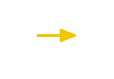
\begin{tikzpicture}[baseline]
    \node [anchor=base] (x) {};
    \draw [rawarrow] (x.mid west) -- ($(x.mid west) + (2em,0)$);
  \end{tikzpicture}
}

\newenvironment{slide}
{\begin{frame}[fragile,environment=slide]\vskip0pt plus 1filll}
{\vskip0pt plus 1filll\end{frame}}

% LaTeX

\setlength{\leftmargini}{1em}

% Common Information

\author{Talia Xu}
\course{COMPSCI 340}
\coursetitle{Operating Systems}
\date{2024 Semester 2}

% fontspec

\defaultfontfeatures{Ligatures=TeX}
% \setmainfont{Domine}
\setsansfont{Inter}[
  FontFace={ul}{n}{Font=*-Thin},
  FontFace={el}{n}{Font=*-ExtraLight},
  FontFace={l}{n}{Font=*-Light},
  FontFace={sb}{n}{Font=*-SemiBold},
  FontFace={eb}{n}{Font=*-ExtraBold},
  FontFace={xb}{n}{Font=*-Black},
]
\setmonofont[Contextuals=AlternateOff, Ligatures=TeXOff]{Iosevka}[
  FontFace={xb}{n}{Font=*-Heavy},
]

%% Font Weights

\DeclareRobustCommand{\ulseries}{\fontseries{ul}\selectfont}
\DeclareTextFontCommand{\textul}{\ulseries}
\DeclareRobustCommand{\elseries}{\fontseries{el}\selectfont}
\DeclareTextFontCommand{\textel}{\elseries}
\DeclareRobustCommand{\lseries}{\fontseries{l}\selectfont}
\DeclareTextFontCommand{\textl}{\lseries}
\DeclareRobustCommand{\sbseries}{\fontseries{sb}\selectfont}
\DeclareTextFontCommand{\textsb}{\sbseries}
\DeclareRobustCommand{\ebseries}{\fontseries{eb}\selectfont}
\DeclareTextFontCommand{\texteb}{\ebseries}
\DeclareRobustCommand{\xbseries}{\fontseries{xb}\selectfont}
\DeclareTextFontCommand{\textxb}{\xbseries}

% tikz

\usetikzlibrary{
  arrows,
  arrows.meta,
  automata,
  backgrounds,
  calc,
  decorations.pathreplacing,
  matrix,
  positioning,
  overlay-beamer-styles,
  shapes,
  shapes.multipart,
  tikzmark,
}

\tikzstyle{rawarrow} = [
  -{Latex[round]},
  line width=1pt,
  yellow,
  shorten >=3pt,
  shorten <=3pt,
  font=\small,
  text=black,
]

\tikzstyle{arrow} = [
  -{Latex[round]},
  line width=1pt,
  yellow,
  shorten >=3pt,
  shorten <=3pt,
  transform canvas={yshift=3pt},
  font=\small,
  text=black,
]

\newcommand{\tikzmarkcoord}[1]{([yshift=3pt]pic cs:#1)}

% minted

\setminted{style=eyolfson, fontsize=\small, escapeinside=||}
\setmintedinline{fontsize=\normalsize}

% hyperref

\hypersetup{colorlinks, urlcolor=blue}

% beamer
\setbeamersize{text margin left=16mm, text margin right=16mm}
\setbeamertemplate{itemize items}[circle]
\setbeamercolor{item}{fg=black}
\setbeamercolor{structure}{fg=darkblue}
\setbeamerfont{frametitle}{series=\bfseries, parent=structure}
\setbeamertemplate{navigation symbols}{}
\setbeamertemplate{headline}{}
\setbeamertemplate{footline}{
  \begin{tikzpicture}[
    remember picture,
    overlay,
    shift={(current page.south west)},
  ]
    \path [fill=gray] (144mm, 0) -- (160mm, 16mm) -- (160mm, 0);
    \node [inner sep=3.5mm, outer sep=0, text=black, anchor=base east,
           align=right, yshift=3.5mm]
          at (current page.south east) {\ttfamily \small \insertframenumber{}};
  \end{tikzpicture}
}
\setbeamertemplate{title page}{
  \begin{tikzpicture}[
    remember picture,
    overlay,
    shift={(current page.south west)},
    background rectangle/.style={fill=darkblue},
    show background rectangle,
  ]
    \node [anchor=center, align=center, text=white, text width=40mm, scale=3.2]
          at (\paperwidth / 2, \paperheight * 2 / 3)
          {\xbseries \inserttitle{}};
    \node [anchor=base west, align=left, inner sep=0, text=white, yshift=2.5mm]
          at (16mm, \paperheight / 3)
          {\insertdate{} \insertcourse{}: \insertcoursetitle{}};
    \node [anchor=base west, align=left, inner sep=0, text=white, yshift=-2.5mm]
          at (16mm, \paperheight / 3)
          {\insertauthor};
    \node [anchor=base east, align=right, inner sep=0, text=white, yshift=2.5mm]
          at (144mm, \paperheight / 3)
          {Lecture \insertlecturenumber{}};
    \node [anchor=base east, align=right, inner sep=0, text=white,
           yshift=-2.5mm]
          at (144mm, \paperheight / 3)
          {\ttfamily \insertversion{}};
    \node [align=center, anchor=south, inner sep=0, text=white, yshift=3.5mm]
          (license) at (\paperwidth / 2, 0)
          {\fontsize{7pt}{7pt}\selectfont This  work is licensed under a
           \href{http://creativecommons.org/licenses/by-sa/4.0/}
                {\color{lightblue} Creative Commons Attribution-ShareAlike 4.0
                 International License}};
  \end{tikzpicture}
}

% xcolor

%% Primary Colour

\definecolor{pantone655}{RGB}{0, 42, 92} % #002a5c
\colorlet{darkblue}{pantone655}

%% Secondary Colours

\definecolor{pantone633}{RGB}{0, 139, 176} % #008bb0
\colorlet{blue}{pantone633}

\definecolor{pantonewarmred}{RGB}{220, 70, 51} % #dc4633
\colorlet{red}{pantonewarmred}

\definecolor{pantone3285}{RGB}{0, 161, 137} % #00a189
\colorlet{cyan}{pantone3285}

\definecolor{pantone7722}{RGB}{13, 83, 77} % #0d534d
\colorlet{darkcyan}{pantone7722}

\definecolor{pantone376}{RGB}{141, 191, 46} % #8dbf2e
\colorlet{green}{pantone376}

\definecolor{pantone2613}{RGB}{109, 36, 122} % #6d247a
\colorlet{violet}{pantone2613}

\definecolor{pantone2985}{RGB}{111, 199, 234} % #6fc7ea
\colorlet{lightblue}{pantone2985}

\definecolor{pantone227}{RGB}{171, 19, 104} % #ab1368
\colorlet{magenta}{pantone227}

\definecolor{pantone7406}{RGB}{241, 197, 0} % #f1c500
\colorlet{yellow}{pantone7406}

%% Neutrals

\definecolor{pantonecoolgray2}{RGB}{208, 209, 201} % #d0d1c9
\colorlet{gray}{pantonecoolgray2}


\lecturenumber{5}
\title{Process Management}
\version{2.0.0}

\begin{document}
  \begin{frame}[plain, noframenumbering]
    \titlepage
  \end{frame}

  \begin{slide}

    \slidetitle{Linux Terminology Is Slightly Different}

    You can look at a process' state by reading \texttt{/proc/<PID>/status | grep State}

    \leftspace{}Replace \texttt{<PID>} with the process ID (or \texttt{self})
    \bigskip

    R: Running and runnable [Running and Waiting]

    S: Interruptible sleep [Blocked]

    D: Uninterruptible sleep [Blocked]

    T: Stopped

    Z: Zombie
    \bigskip

    The kernel lets you explicitly stop a process to prevent it from running

    \leftspace{}You or another process must explicitly continue it

  \end{slide}

  \begin{slide}
    \slidetitle{On Unix, the Kernel Launches A Single User Process}

    After the kernel initializes, it creates a single process
    from a program
    \bigskip


    This process is called \texttt{init}, and it looks for it in \texttt{/sbin/init}

    \leftspace{}Responsible for executing every other process on the machine

    \leftspace{}Must always be active, if it exits the kernel thinks you're shutting down
    \bigskip

    For Linux, \texttt{init} will probably be \texttt{systemd} but there's other options
    \bigskip

    Aside: some operating systems create an ``idle'' process that the
    scheduler can run
  \end{slide}

  \begin{slide}

    \slidetitle{A Typical Process Tree on the Virtual Machine}

    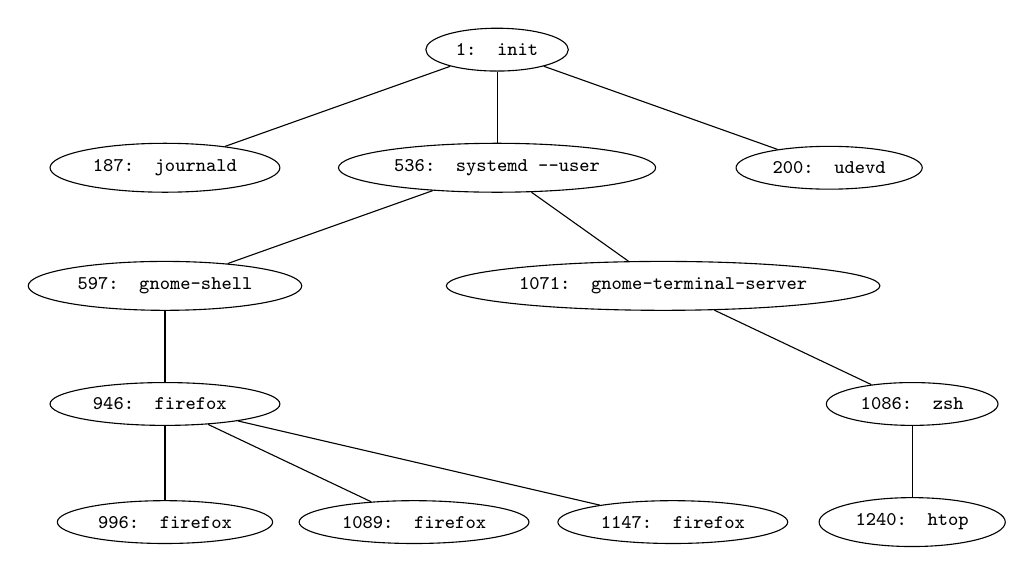
\begin{tikzpicture}[sibling distance=12em]
      \tikzstyle{every node}=[ellipse, draw, font=\scriptsize\ttfamily, align=center]
      \node {1: init}
        child { node {187: journald} }
        child { node {536: systemd --user}
          child { node [xshift=-6em] {597: gnome-shell}
            child { node { 946: firefox }
              child { node [xshift=12em] {996: firefox} }
              child { node [xshift=9em] {1089: firefox} }
              child { node [xshift=6.35em] {1147: firefox} }
            }
          }
          child { node {1071: gnome-terminal-server}
            child { node [xshift=9em] {1086: zsh}
              child { node {1240: htop}
              }
            }
          }
        }
        child { node {200: udevd} };
    \end{tikzpicture}

  \end{slide}

  \begin{slide}

    \slidetitle{How You Can See Your Process Tree}

    Use \texttt{htop}
    \bigskip

    You can press \texttt{F5} to switch between tree and list view

  \end{slide}

  \begin{slide}

    \slidetitle{Processes Are Assigned a Process ID (pid) On Creation and Does
                Not Change}

    The process ID is just a number, and is unique for every \textbf{active}
    process
    \bigskip

    On most Linux systems the maximum pid 32768, and 0 is reserved (invalid)
    \bigskip

    Eventually the kernel will recycle a pid, after the process dies, for a new process
    \bigskip

    Remember: each process has its own \textit{address space} (independent view of memory)

  \end{slide}

  \begin{slide}

    \slidetitle{Maintaining the Parent/Child Relationship}

    Previously, we made sure that our parent exited last (by using \texttt{sleep})
    \bigskip

    What happens if the parent process exits first, and no longer exists?

  \end{slide}

  \begin{slide}

    \slidetitle{The Parent Process is Responsible for Its Child}

    The operating system sets the exit status when a process terminates

    (the process terminates by calling \texttt{exit})

    \leftspace{}It can't remove its PCB yet
    \bigskip

    The minimum acknowledgment the parent has to do is read the child's exit status
    \bigskip

    There's two situations:
    \begin{enumerate}
      \item The child exits first (zombie process)
      \item The parent exits first (orphan process)
    \end{enumerate}

  \end{slide}

  \begin{slide}

    \slidetitle{You Need to Call \texttt{\bfseries wait} on Child Processes}

    \texttt{wait} as the following API:
    \begin{itemize}
      \item \texttt{status}: Address to store the wait status of the process
      \item Returns the process ID of child process

            \leftspace{}-1: on failure

            \leftspace{}0: for non blocking calls with no child changes

            \leftspace{}>0: the child with a change
    \end{itemize}
    \bigskip

    The wait status contains a bunch of information, including the exit code

    \leftspace{}Use \texttt{man wait} to find all the macros to query wait status

    \leftspace{}\leftspace{}You can use \texttt{waitpid} to wait on a specific child process

  \end{slide}

  \begin{slide}

    \slidetitle{
      \texttt{\bfseries wait-example.c} Blocks Until The Child Process Exits,
      and Cleans Up
    }

    \begin{minted}{c}
int main(int argc, char *argv[]) {
  pid_t pid = fork();
  if (pid == -1) { return errno; }
  if (pid == 0) {
    sleep(2);
  }
  else {
    printf("Calling wait\n");
    int wstatus;
    pid_t wait_pid = wait(&wstatus);
    if (WIFEXITED(wstatus)) {
      printf("Wait returned for an exited process! pid: %d, status: %d\n",
             wait_pid, WEXITSTATUS(wstatus));
    }
  }
  return 0;
}
    \end{minted}

  \end{slide}

  \begin{slide}

    \slidetitle{A Zombie Process Waits for Its Parent to Read Its Exit Status}

    The process is terminated, but it hasn't been acknowledged
    \medskip

    A process may have an error in it, where it never reads the child's exit status
    \medskip

    The operating system can interrupt the parent process to acknowledge the child

    \leftspace{}It is just a suggestion and the parent is free to ignore it

    \leftspace{}\leftspace{}This is a basic form of IPC called a signal
    \bigskip

    The operating system has to keep a zombie process until it's acknowledged

    \leftspace{}If the parent ignores it, the zombie process needs to wait to
    be re-parented
  \end{slide}

  \begin{slide}

    \slidetitle{An Orphan Process Needs a New Parent}

    The child process lost its parent process

    \leftspace{}The child still needs a process to acknowledge its exit
    \medskip

    The operating system re-parents the child process to \texttt{init}

    \leftspace{}The \texttt{init} process is now responsible to acknowledge the
                 child
  \end{slide}

  \begin{slide}

    \slidetitle{
      \texttt{\bfseries orphan-example.c} The Parent Exits Before the Child,
      \texttt{init} Cleans Up
    }

    \begin{minted}{c}
int main(int argc, char *argv[]) {
  pid_t pid = fork();
  if (pid == -1) {
    int err = errno;
    perror("fork failed");
    return err;
  }
  if (pid == 0) {
    printf("Child parent pid: %d\n", getppid());
    sleep(2);
    printf("Child parent pid (after sleep): %d\n", getppid());
  }
  else {
    sleep(1);
  }
  return 0;
}

    \end{minted}

  \end{slide}

  \begin{slide}

    \slidetitle{
      \texttt{\bfseries zombie-example.c} The Parent Monitors the Child To Check
      Its State
    }

    \begin{minted}{c}
  pid_t pid = fork();
  // Error checking
  if (pid == 0) {
    sleep(2);
  }
  else {
    // Parent process
    int ret;
    sleep(1);
    printf("Child process state: ");
    ret = print_state(pid);
    if (ret < 0) { return errno; }
    sleep(2);
    printf("Child process state: ");
    ret = print_state(pid);
    if (ret < 0) { return errno; }
  }
    \end{minted}

  \end{slide}

  \begin{slide}

    \slidetitle{You're Responsible for Managing Processes}

    The operating system maintains a strict parent/child relationship
    \medskip
    
    You should be able to identify (and prevent) the following:
    \begin{itemize}
      \item Zombie processes
      \item Orphan processes
    \end{itemize}
  \end{slide}
\end{document}
